%\color{ForestGreen}
\chapter{Layout Guidelines for an \ERm}
\label{chp:layout}

\section{Introduction}

The previous chapters describe the appearance and meaning of \SBGNERLone components which are \glyph{entity nodes} as well as \glyph{relationships}. The components of an \ERm have to be placed in a meaningful way -- a random distribution with spaghetti-like connections will most likely hide the information encoded in the underlying model, whereas an elegant placement of the objects, giving a congenial appearance of the maps, may reveal new insights. The arrangement of components in a map is called a \emph{layout}.

SBGN \ERms should be easily recognizable not only by the glyphs used, but also by the general style of the layout. However, the arrangement of the components is a complex art in itself, and there is no simple rule which can be applied to all cases. Therefore this section provides guidelines for the layout of \ERs, divided into two categories:
\begin{enumerate}
  \item requirements, i.\,e.~rules which \textbf{must} be fulfilled by a layout, and
  \item recommendations, i.\,e.~rules which \textbf{should} be followed if possible.
\end{enumerate}
In addition, we provide a list of additional suggestions which may help in producing aesthetically more pleasant layouts, possibly easier to understand.

Those layout guidelines are independent of the method used to produce the map, and apply to both manually drawn maps as well as maps produced by an automatic layout algorithm. The guidelines do not deal with interactive aspects (e.\,g.~the effect of zooming). Further information about automatic network layout (graph drawing) can be found, for example, in the books of Di Battista and co-authors~\cite{DiBattista:1998} and Kaufmann and Wagner~\cite{Kaufmann:2001}.

Please note that the color of objects do not carry any meaning in SBGN. Although one can use colors to emphasize part of a map or encode additional information, the meaning of the map should not depend on the colors. Furthermore, objects can have different sizes and size is also meaningless in SBGN. For example, a transition node may be larger than a protein node. Also the meaning of a graph should be conserved upon scaling as far as possible.

\newpage

\section{Layout guidelines}

\subsection{Requirements}

Requirements are rules which \textbf{must} be fulfilled by a layout to produce a valid \SBGNERLone graph.

\subsubsection{Node-node overlaps}

Nodes are only allowed to overlap in the case that the overlapping nodes define a glyph. Examples are stacking auxiliary items such as an \glyph{unit of information} on top of an \glyph{entity}, or an \glyph{interaction} and nesting \glyph{entities} to represent domains (\sect{domain}). In other cases, nodes are not allowed to overlap (\fig{layout1}). This includes the touching of nodes. 

\begin{figure}[h!]
  \centering
  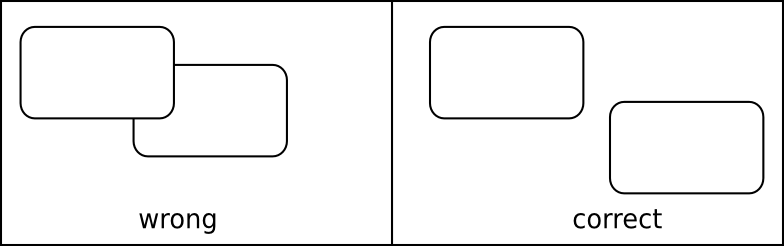
\includegraphics[scale=0.3]{images/layout-node-node}
  \caption{Nodes must not overlap.}\label{fig:layout1}
\end{figure}

In the case of domain nesting, the internal \glyph{entities} must be completely included in the enclosing \glyph{entities}.

\subsubsection{Node-edge crossing}\label{crosEdNoRe}

In case of node-edge crossing the edge must be drawn on the top of the node (\fig{layout2}). See also recommendation \ref{crosEdNo} (crossing between edges and nodes should be avoided).

\begin{figure}[h!]
  \centering
  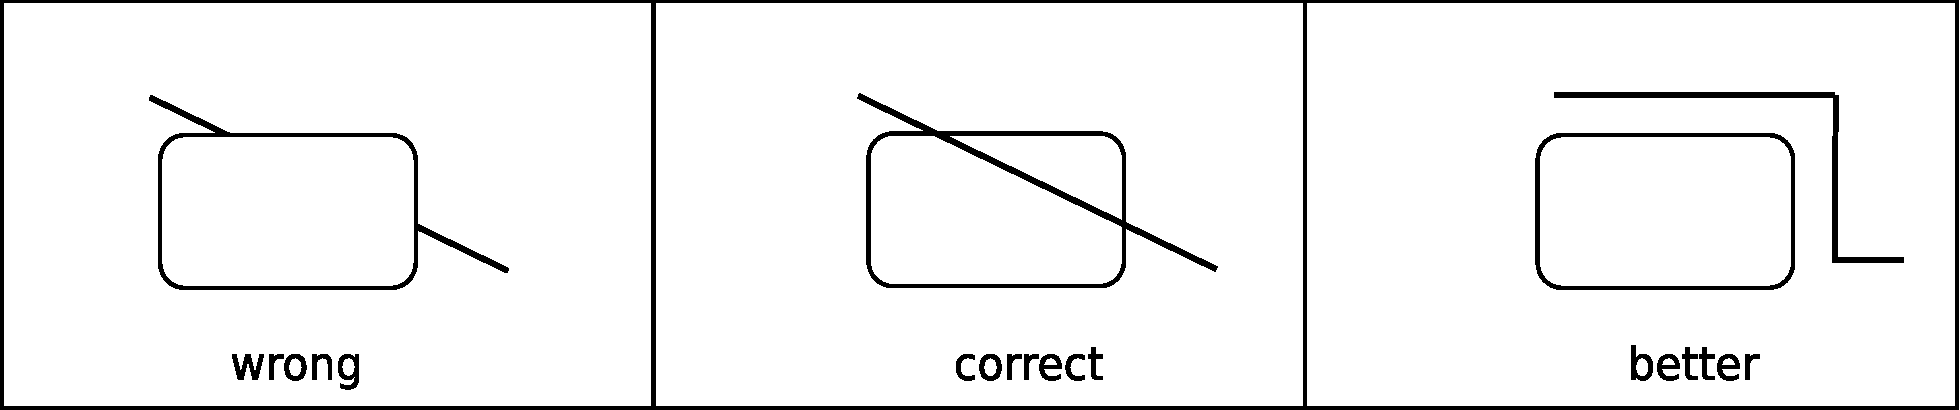
\includegraphics[scale=0.3]{images/layout-node-edge}
  \caption{If an edge crosses a node, the edge must be drawn on top of the node.}\label{fig:layout2}
\end{figure}

\subsubsection{Node border-edge overlaps}

Edges are not allowed to overlap the border lines of nodes (\fig{layout3}).

\begin{figure}[h!]
  \centering
  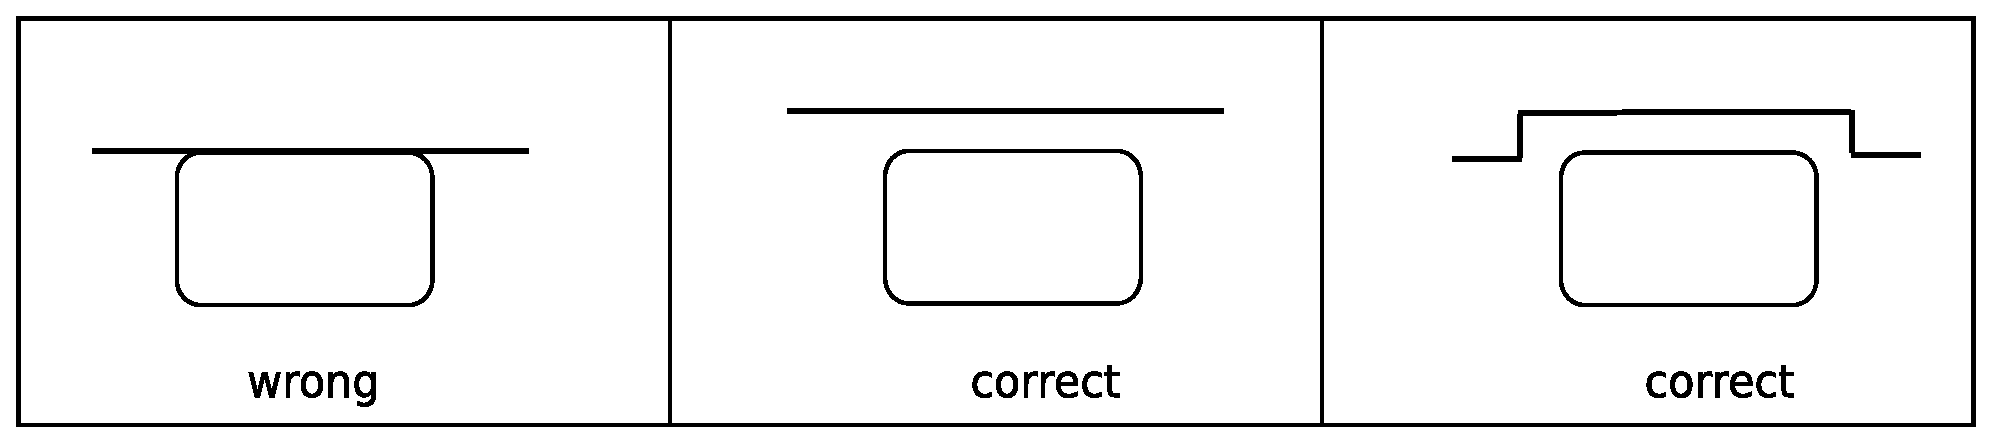
\includegraphics[scale=0.3]{images/layout-node-border-edge}
  \caption{Edges must not overlap node borders.}\label{fig:layout3}
\end{figure}

\subsubsection{Edge-edge overlaps}

Edges are not allowed to overlap (\fig{layout4}). This includes touching of edges. Furthermore, an edge is neither allowed to cross itself nor to cross a boundary of node more than twice or other edges more than once.

\begin{figure}[h!]
  \centering
  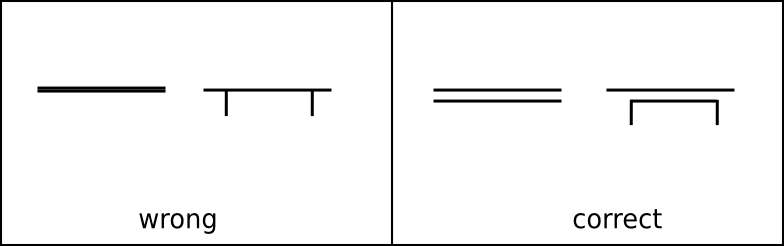
\includegraphics[scale=0.3]{images/layout-edge-edge}
  \caption{Edges must not overlap.}\label{fig:layout4}
\end{figure}

\subsubsection{Node orientation}

Nodes have to be drawn horizontally or vertically, any other rotation of elements is not allowed (\fig{layout5}).

\begin{figure}[h!]
  \centering
  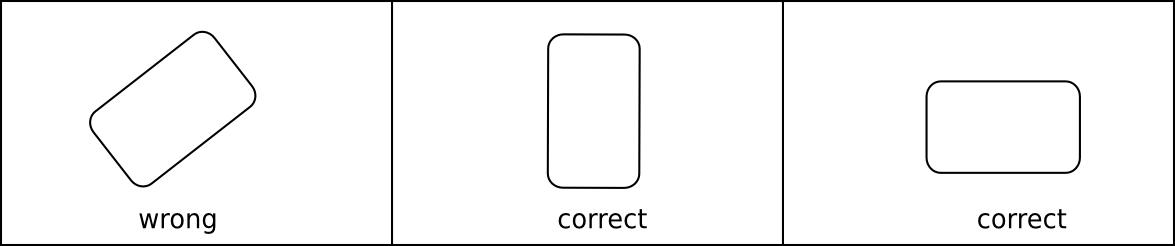
\includegraphics[scale=0.3]{images/layout-orientation}
  \caption{The node orientation must be horizontally or vertically.}\label{fig:layout5}
\end{figure}

\subsubsection{Interactions}

The \glyph{interaction arcs} linking more than two \glyph{interactor nodes} are attached to a circle. Several outcomes of an interaction are not allowed to overlap (\fig{layout6}).

\begin{figure}[h!]
  \centering
  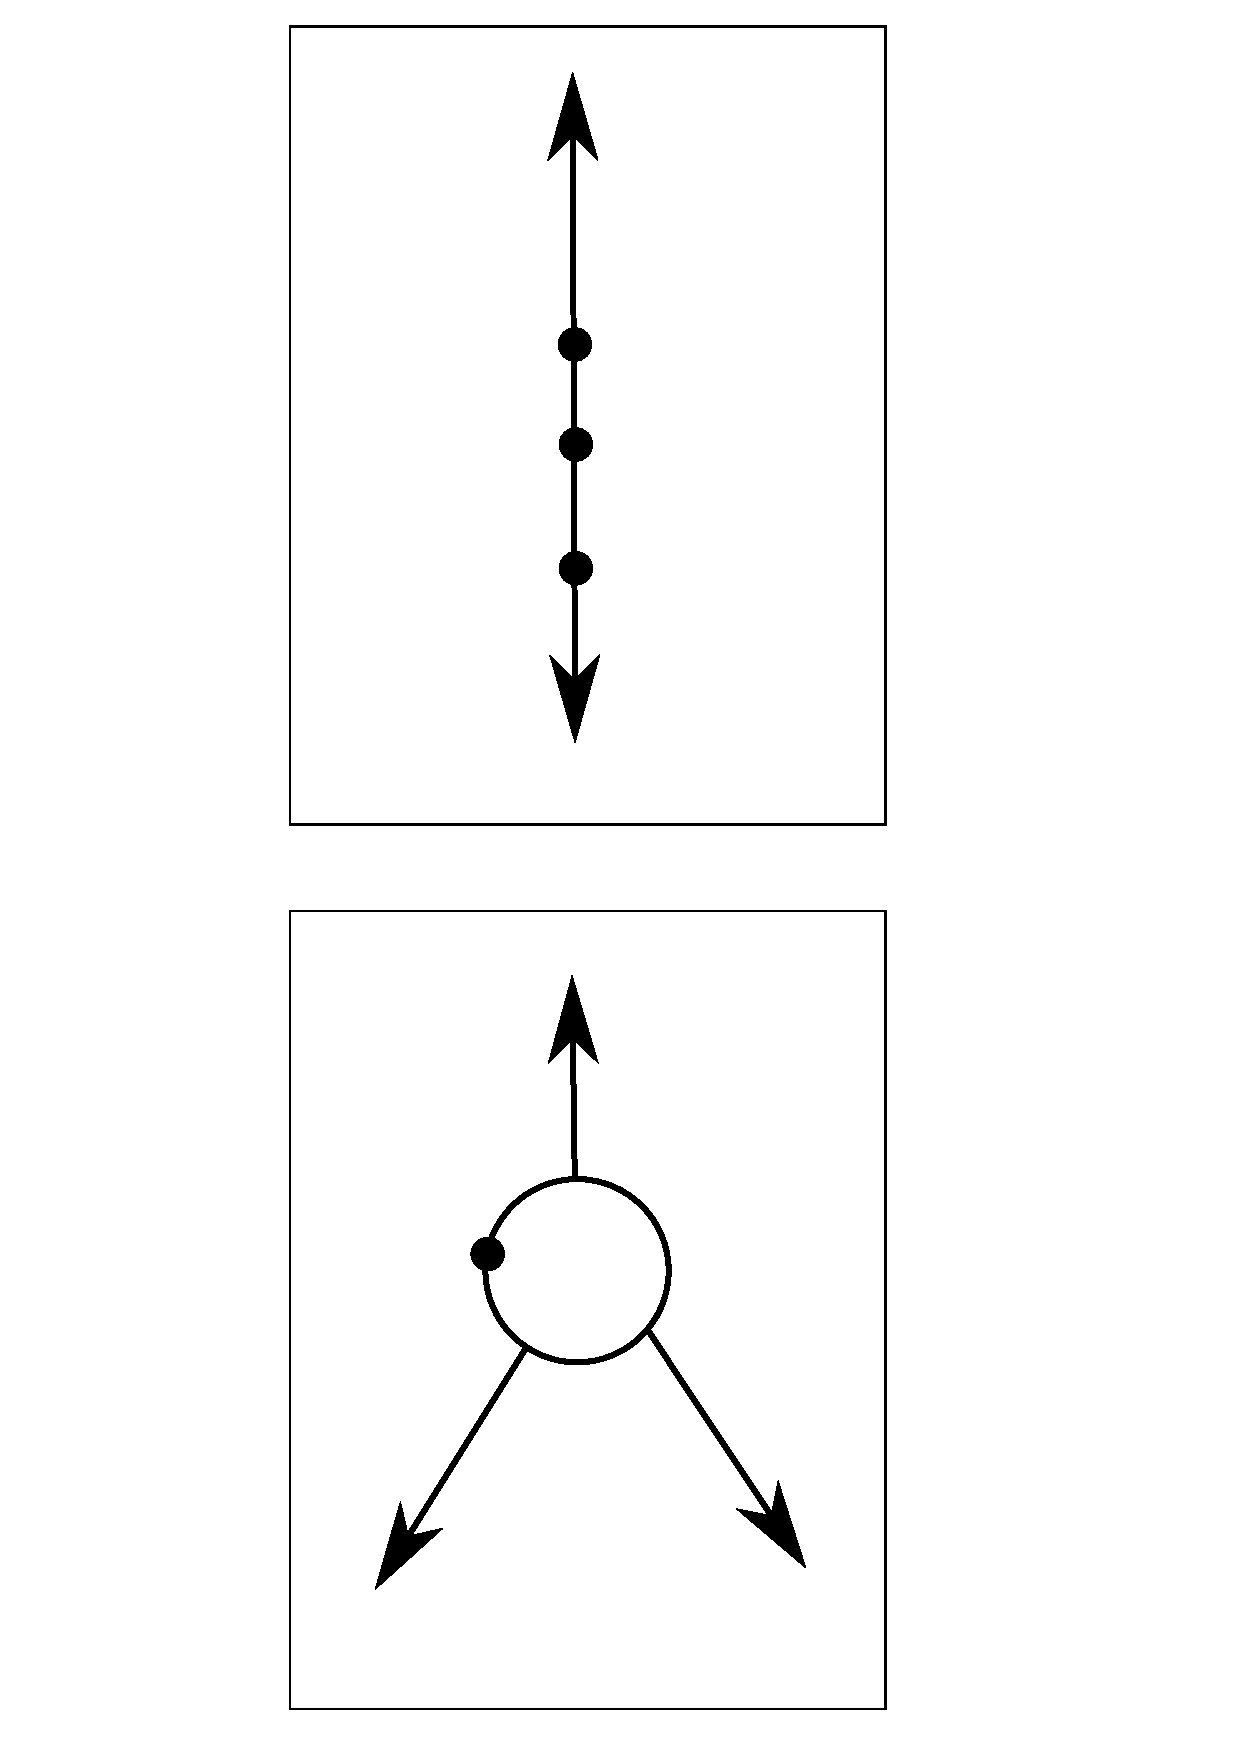
\includegraphics[scale=0.3]{images/layout-connecting-arcs}
  \caption{Arcs linking more than two \glyph{interactor nodes} are attached to a circle and outcomes of an interaction are not allowed to overlap.}\label{fig:layout6}
\end{figure}

\subsubsection{Node labels}

At least a part of the label (unbordered box containing a string of characters) has to be placed inside the node it belongs to. Node labels are not allowed to overlap nodes or other labels (this includes touching of other nodes or labels).

\subsubsection{Edge labels}

Edge labels are not allowed to overlap nodes. This includes touching of nodes.

\subsubsection{Annotation links}

The links between an annotation and the annotated element should be clearly different from the relationships. They can be callouts, thick edges, dashed edges etc. as long as they differ from the continuous lines used for statements and influences.

\subsection{Recommendations}

Recommendations are rules which should be followed if possible to produce layouts may be easier to understand.

\subsubsection{Multiple \glyph{entities} to represent the same concept}\label{multEnt}

Because rules (the influence of one entity node on a relationship) are independent of each other, a given ``entity'' (the concept) can be represented by many \glyph{entities} (the symbols). If a map is particularly large and an entity highly influenced or influential, it may be a good idea to represent the entity several time, limiting the influences to or from each instance. However, if systematised, such a procedure would lead to disconnected maps difficult to read and interpret. It is recommended to adopt a parsimonious approach, and multiply the symbols representing an entity only when the map become unreadable without doing so.

\subsubsection{Node-edge crossing}\label{crosEdNo}

Crossings between edges and nodes should be avoided. See also requirement \ref{crosEdNoRe} (in case of node-edge crossings the edge must be drawn on the top of the node).

\begin{figure}[h!]
  \centering
  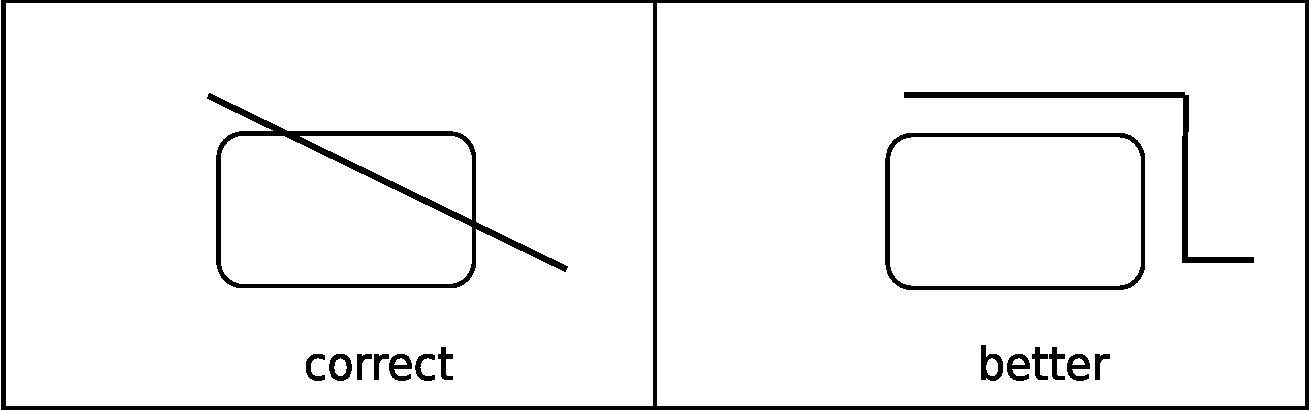
\includegraphics[scale=0.3]{images/layout-node-edge-2}
  \caption{Edges should not cross node.}\label{fig:layout7}
\end{figure}


\subsubsection{Labels}

Labels should be horizontal. Node labels should be placed completely inside the node if possible. Edge labels should be placed close to the edge and avoid overlapping the edge as well as other edge labels.

\subsubsection{Avoid edge crossings}

The amount of crossings between edges should be minimized.

\subsubsection{Units of information}

Units of information should not hide the structure of the corresponding node and should not overlap other elements.

\subsection{Additional suggestions}

Here is a list of additional layout suggestions which may help in producing aesthetically more pleasing layouts which may be easier to understand.

\begin{itemize}
  \item Angle of edge crossings: If edge crossings are not avoidable edges should cross with an angle close to 90 degrees.
  \item Drawing area and width/height ratio: The drawing should be compact and the ratio between the width and the height of the drawing should be close to 1.
  \item Edge length: Long edges should be avoided.
  \item Number of edge bends: Edges should be drawn with as few bends as possible.
  \item Similar and symmetric parts: Similar parts of a map should be drawn in a similar way, and symmetric parts should be drawn symmetrically.
  \item Proximity information: Related elements (e.\,g.~nodes connected by an arc or all elements within a submap) should be drawn close together.
\end{itemize} 

%\normalcolor